% Options for packages loaded elsewhere
\PassOptionsToPackage{unicode}{hyperref}
\PassOptionsToPackage{hyphens}{url}
%
\documentclass[
]{article}
\usepackage{amsmath,amssymb}
\usepackage{lmodern}
\usepackage{ifxetex,ifluatex}
\ifnum 0\ifxetex 1\fi\ifluatex 1\fi=0 % if pdftex
  \usepackage[T1]{fontenc}
  \usepackage[utf8]{inputenc}
  \usepackage{textcomp} % provide euro and other symbols
\else % if luatex or xetex
  \usepackage{unicode-math}
  \defaultfontfeatures{Scale=MatchLowercase}
  \defaultfontfeatures[\rmfamily]{Ligatures=TeX,Scale=1}
\fi
% Use upquote if available, for straight quotes in verbatim environments
\IfFileExists{upquote.sty}{\usepackage{upquote}}{}
\IfFileExists{microtype.sty}{% use microtype if available
  \usepackage[]{microtype}
  \UseMicrotypeSet[protrusion]{basicmath} % disable protrusion for tt fonts
}{}
\makeatletter
\@ifundefined{KOMAClassName}{% if non-KOMA class
  \IfFileExists{parskip.sty}{%
    \usepackage{parskip}
  }{% else
    \setlength{\parindent}{0pt}
    \setlength{\parskip}{6pt plus 2pt minus 1pt}}
}{% if KOMA class
  \KOMAoptions{parskip=half}}
\makeatother
\usepackage{xcolor}
\IfFileExists{xurl.sty}{\usepackage{xurl}}{} % add URL line breaks if available
\IfFileExists{bookmark.sty}{\usepackage{bookmark}}{\usepackage{hyperref}}
\hypersetup{
  pdftitle={Comment and Working Paper Figures and Tables not created elsewhere},
  hidelinks,
  pdfcreator={LaTeX via pandoc}}
\urlstyle{same} % disable monospaced font for URLs
\usepackage[margin=1in]{geometry}
\usepackage{color}
\usepackage{fancyvrb}
\newcommand{\VerbBar}{|}
\newcommand{\VERB}{\Verb[commandchars=\\\{\}]}
\DefineVerbatimEnvironment{Highlighting}{Verbatim}{commandchars=\\\{\}}
% Add ',fontsize=\small' for more characters per line
\usepackage{framed}
\definecolor{shadecolor}{RGB}{248,248,248}
\newenvironment{Shaded}{\begin{snugshade}}{\end{snugshade}}
\newcommand{\AlertTok}[1]{\textcolor[rgb]{0.94,0.16,0.16}{#1}}
\newcommand{\AnnotationTok}[1]{\textcolor[rgb]{0.56,0.35,0.01}{\textbf{\textit{#1}}}}
\newcommand{\AttributeTok}[1]{\textcolor[rgb]{0.77,0.63,0.00}{#1}}
\newcommand{\BaseNTok}[1]{\textcolor[rgb]{0.00,0.00,0.81}{#1}}
\newcommand{\BuiltInTok}[1]{#1}
\newcommand{\CharTok}[1]{\textcolor[rgb]{0.31,0.60,0.02}{#1}}
\newcommand{\CommentTok}[1]{\textcolor[rgb]{0.56,0.35,0.01}{\textit{#1}}}
\newcommand{\CommentVarTok}[1]{\textcolor[rgb]{0.56,0.35,0.01}{\textbf{\textit{#1}}}}
\newcommand{\ConstantTok}[1]{\textcolor[rgb]{0.00,0.00,0.00}{#1}}
\newcommand{\ControlFlowTok}[1]{\textcolor[rgb]{0.13,0.29,0.53}{\textbf{#1}}}
\newcommand{\DataTypeTok}[1]{\textcolor[rgb]{0.13,0.29,0.53}{#1}}
\newcommand{\DecValTok}[1]{\textcolor[rgb]{0.00,0.00,0.81}{#1}}
\newcommand{\DocumentationTok}[1]{\textcolor[rgb]{0.56,0.35,0.01}{\textbf{\textit{#1}}}}
\newcommand{\ErrorTok}[1]{\textcolor[rgb]{0.64,0.00,0.00}{\textbf{#1}}}
\newcommand{\ExtensionTok}[1]{#1}
\newcommand{\FloatTok}[1]{\textcolor[rgb]{0.00,0.00,0.81}{#1}}
\newcommand{\FunctionTok}[1]{\textcolor[rgb]{0.00,0.00,0.00}{#1}}
\newcommand{\ImportTok}[1]{#1}
\newcommand{\InformationTok}[1]{\textcolor[rgb]{0.56,0.35,0.01}{\textbf{\textit{#1}}}}
\newcommand{\KeywordTok}[1]{\textcolor[rgb]{0.13,0.29,0.53}{\textbf{#1}}}
\newcommand{\NormalTok}[1]{#1}
\newcommand{\OperatorTok}[1]{\textcolor[rgb]{0.81,0.36,0.00}{\textbf{#1}}}
\newcommand{\OtherTok}[1]{\textcolor[rgb]{0.56,0.35,0.01}{#1}}
\newcommand{\PreprocessorTok}[1]{\textcolor[rgb]{0.56,0.35,0.01}{\textit{#1}}}
\newcommand{\RegionMarkerTok}[1]{#1}
\newcommand{\SpecialCharTok}[1]{\textcolor[rgb]{0.00,0.00,0.00}{#1}}
\newcommand{\SpecialStringTok}[1]{\textcolor[rgb]{0.31,0.60,0.02}{#1}}
\newcommand{\StringTok}[1]{\textcolor[rgb]{0.31,0.60,0.02}{#1}}
\newcommand{\VariableTok}[1]{\textcolor[rgb]{0.00,0.00,0.00}{#1}}
\newcommand{\VerbatimStringTok}[1]{\textcolor[rgb]{0.31,0.60,0.02}{#1}}
\newcommand{\WarningTok}[1]{\textcolor[rgb]{0.56,0.35,0.01}{\textbf{\textit{#1}}}}
\usepackage{longtable,booktabs,array}
\usepackage{calc} % for calculating minipage widths
% Correct order of tables after \paragraph or \subparagraph
\usepackage{etoolbox}
\makeatletter
\patchcmd\longtable{\par}{\if@noskipsec\mbox{}\fi\par}{}{}
\makeatother
% Allow footnotes in longtable head/foot
\IfFileExists{footnotehyper.sty}{\usepackage{footnotehyper}}{\usepackage{footnote}}
\makesavenoteenv{longtable}
\usepackage{graphicx}
\makeatletter
\def\maxwidth{\ifdim\Gin@nat@width>\linewidth\linewidth\else\Gin@nat@width\fi}
\def\maxheight{\ifdim\Gin@nat@height>\textheight\textheight\else\Gin@nat@height\fi}
\makeatother
% Scale images if necessary, so that they will not overflow the page
% margins by default, and it is still possible to overwrite the defaults
% using explicit options in \includegraphics[width, height, ...]{}
\setkeys{Gin}{width=\maxwidth,height=\maxheight,keepaspectratio}
% Set default figure placement to htbp
\makeatletter
\def\fps@figure{htbp}
\makeatother
\setlength{\emergencystretch}{3em} % prevent overfull lines
\providecommand{\tightlist}{%
  \setlength{\itemsep}{0pt}\setlength{\parskip}{0pt}}
\setcounter{secnumdepth}{-\maxdimen} % remove section numbering
\ifluatex
  \usepackage{selnolig}  % disable illegal ligatures
\fi

\title{Comment and Working Paper Figures and Tables not created
elsewhere}
\author{}
\date{\vspace{-2.5em}}

\begin{document}
\maketitle

\hypertarget{basic-statistics}{%
\section{0 Basic statistics}\label{basic-statistics}}

\hypertarget{share-of-reported-mu-sigma-t-p-and-ci}{%
\subsubsection{Share of reported mu / sigma, t, p and
CI}\label{share-of-reported-mu-sigma-t-p-and-ci}}

\begin{longtable}[]{@{}lrr@{}}
\toprule
report & n & share \\
\midrule
\endhead
ci & 23 & 0.0010580 \\
p & 1014 & 0.0466421 \\
s & 19618 & 0.9023919 \\
t & 1085 & 0.0499080 \\
\bottomrule
\end{longtable}

\hypertarget{the-rounding-problem-and-our-solution-in-the-pooled-data}{%
\section{1 The rounding problem and our solution in the pooled
data}\label{the-rounding-problem-and-our-solution-in-the-pooled-data}}

\hypertarget{figure-1-combined-in-two-panels}{%
\subsubsection{Figure 1 Combined in Two
panels}\label{figure-1-combined-in-two-panels}}

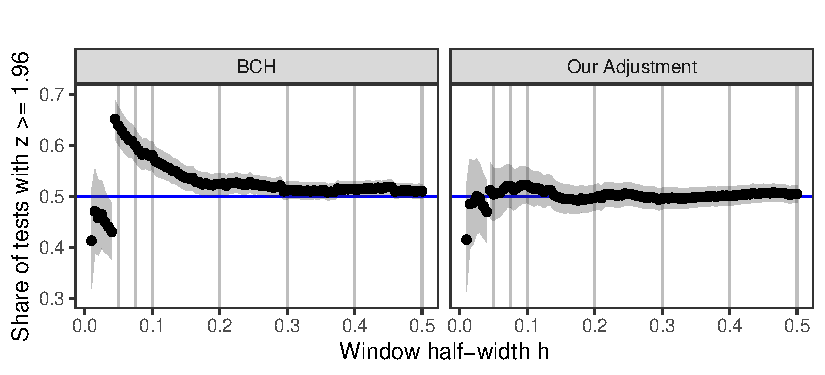
\includegraphics{C:/Users/ppuetz/Desktop/sciebo/methods_matter_replication/Submission AER/revision/comment_methods_matter/replication_repo_methods_matter_comment/Results/share_of_significant_tests-1.pdf}

\hypertarget{figure-2-number-of-included-observations}{%
\subsubsection{Figure 2: Number of included
observations}\label{figure-2-number-of-included-observations}}

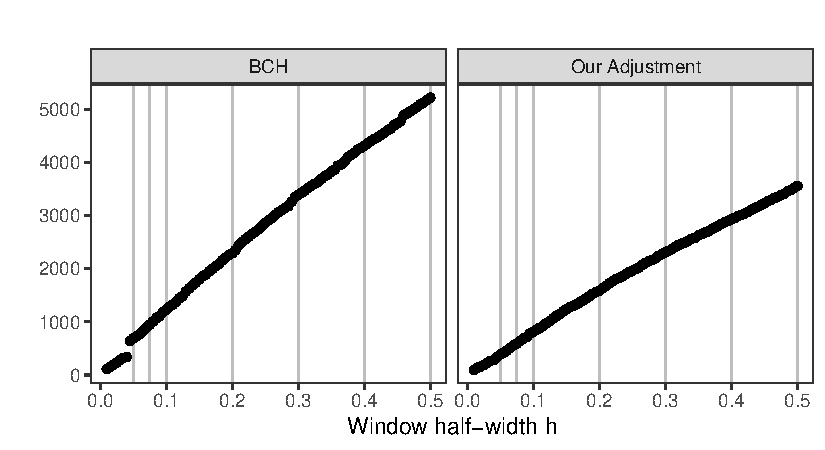
\includegraphics{C:/Users/ppuetz/Desktop/sciebo/methods_matter_replication/Submission AER/revision/comment_methods_matter/replication_repo_methods_matter_comment/Results/number_of_included_observations-1.pdf}

\hypertarget{share-of-obs-with-z2-in-smallest-window}{%
\subsubsection{Share of obs with z==2 in smallest
window}\label{share-of-obs-with-z2-in-smallest-window}}

\begin{Shaded}
\begin{Highlighting}[]
\FunctionTok{sum}\NormalTok{(dat}\SpecialCharTok{$}\NormalTok{z}\SpecialCharTok{==}\DecValTok{2}\NormalTok{, }\AttributeTok{na.rm=}\ConstantTok{TRUE}\NormalTok{)}
\end{Highlighting}
\end{Shaded}

\begin{verbatim}
## [1] 260
\end{verbatim}

\begin{Shaded}
\begin{Highlighting}[]
\NormalTok{d }\OtherTok{=} \FunctionTok{filter}\NormalTok{(dat, }\FunctionTok{abs}\NormalTok{(z}\FloatTok{{-}1.96}\NormalTok{)}\SpecialCharTok{\textless{}=}\FloatTok{0.05}\NormalTok{)}
\FunctionTok{sum}\NormalTok{(d}\SpecialCharTok{$}\NormalTok{z}\SpecialCharTok{==}\DecValTok{2}\NormalTok{, }\AttributeTok{na.rm=}\ConstantTok{TRUE}\NormalTok{)}
\end{Highlighting}
\end{Shaded}

\begin{verbatim}
## [1] 260
\end{verbatim}

\begin{Shaded}
\begin{Highlighting}[]
\FunctionTok{sum}\NormalTok{(d}\SpecialCharTok{$}\NormalTok{z}\SpecialCharTok{==}\DecValTok{2}\NormalTok{, }\AttributeTok{na.rm=}\ConstantTok{TRUE}\NormalTok{) }\SpecialCharTok{/} \FunctionTok{NROW}\NormalTok{(d)}
\end{Highlighting}
\end{Shaded}

\begin{verbatim}
## [1] 0.3790087
\end{verbatim}

\hypertarget{table-of-significant-digits-of-standard-error}{%
\subsection{Table of significant digits of standard
error}\label{table-of-significant-digits-of-standard-error}}

\hypertarget{share-digits}{%
\subsubsection{Share digits}\label{share-digits}}

\begin{longtable}[]{@{}lrll@{}}
\toprule
subset & obs & single\_signif\_sd & single\_or\_double\_signif\_sd \\
\midrule
\endhead
z is 2 & 260 & 68.6\% & 97.7\% \\
z is not 2 & 21480 & 17.2\% & 59.8\% \\
\bottomrule
\end{longtable}

\hypertarget{correlation-s-37-and-z}{%
\subsubsection{Correlation s \textless= 37 and
z}\label{correlation-s-37-and-z}}

\begin{Shaded}
\begin{Highlighting}[]
\FunctionTok{cor.test}\NormalTok{(dat}\SpecialCharTok{$}\NormalTok{z, 1L}\SpecialCharTok{*}\NormalTok{(}\SpecialCharTok{!}\NormalTok{dat}\SpecialCharTok{$}\NormalTok{keep.obs))}
\end{Highlighting}
\end{Shaded}

\begin{verbatim}
## 
##  Pearson's product-moment correlation
## 
## data:  dat$z and 1L * (!dat$keep.obs)
## t = -0.77946, df = 21738, p-value = 0.4357
## alternative hypothesis: true correlation is not equal to 0
## 95 percent confidence interval:
##  -0.018578286  0.008006953
## sample estimates:
##          cor 
## -0.005286601
\end{verbatim}

\begin{Shaded}
\begin{Highlighting}[]
\NormalTok{dat.omit }\OtherTok{=}\NormalTok{ dat }\SpecialCharTok{\%\textgreater{}\%} \FunctionTok{select}\NormalTok{(mu,z, sigma) }\SpecialCharTok{\%\textgreater{}\%} \FunctionTok{filter}\NormalTok{(}\FunctionTok{is.finite}\NormalTok{(z), }\FunctionTok{is.finite}\NormalTok{(sigma))}
\FunctionTok{cor.test}\NormalTok{(dat.omit}\SpecialCharTok{$}\NormalTok{z, dat.omit}\SpecialCharTok{$}\NormalTok{sigma)}
\end{Highlighting}
\end{Shaded}

\begin{verbatim}
## 
##  Pearson's product-moment correlation
## 
## data:  dat.omit$z and dat.omit$sigma
## t = -0.025255, df = 20608, p-value = 0.9799
## alternative hypothesis: true correlation is not equal to 0
## 95 percent confidence interval:
##  -0.01382844  0.01347666
## sample estimates:
##           cor 
## -0.0001759225
\end{verbatim}

\begin{Shaded}
\begin{Highlighting}[]
\NormalTok{dat.omit }\OtherTok{=} \FunctionTok{filter}\NormalTok{(dat.omit,z }\SpecialCharTok{\textgreater{}}\DecValTok{0}\NormalTok{, sigma }\SpecialCharTok{\textgreater{}} \DecValTok{0}\NormalTok{)}
\FunctionTok{cor.test}\NormalTok{(}\FunctionTok{log}\NormalTok{(dat.omit}\SpecialCharTok{$}\NormalTok{z), dat.omit}\SpecialCharTok{$}\NormalTok{sigma)}
\end{Highlighting}
\end{Shaded}

\begin{verbatim}
## 
##  Pearson's product-moment correlation
## 
## data:  log(dat.omit$z) and dat.omit$sigma
## t = 0.13898, df = 20395, p-value = 0.8895
## alternative hypothesis: true correlation is not equal to 0
## 95 percent confidence interval:
##  -0.01275066  0.01469661
## sample estimates:
##          cor 
## 0.0009731582
\end{verbatim}

\hypertarget{table-of-omitted-obs}{%
\subsubsection{Table of omitted obs}\label{table-of-omitted-obs}}

\begin{longtable}[]{@{}lrl@{}}
\toprule
group & count & share.omit \\
\midrule
\endhead
z=2 & 260 & 87.3\% \\
other bunching & 4212 & 81.1\% \\
no bunching & 17268 & 26.6\% \\
\bottomrule
\end{longtable}

\begin{longtable}[]{@{}rl@{}}
\toprule
count & share.omit \\
\midrule
\endhead
21740 & 37.9\% \\
\bottomrule
\end{longtable}

\begin{verbatim}
## Loading required package: stringr
\end{verbatim}

\begin{verbatim}
## 
## Attaching package: 'stringtools'
\end{verbatim}

\begin{verbatim}
## The following objects are masked from 'package:RoundingMatters':
## 
##     str.between, str.left.of, str.right.of
\end{verbatim}

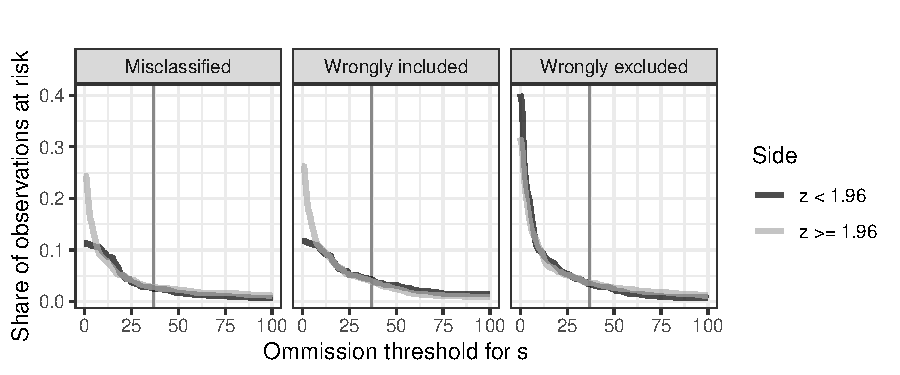
\includegraphics{C:/Users/ppuetz/Desktop/sciebo/methods_matter_replication/Submission AER/revision/comment_methods_matter/replication_repo_methods_matter_comment/Results/observations_at_risk-1.pdf}

\hypertarget{table-of-most-common-bunched-z-values}{%
\subsubsection{Table of most common bunched
z-values}\label{table-of-most-common-bunched-z-values}}

\hypertarget{counts-by-method}{%
\section{Counts by method}\label{counts-by-method}}

\begin{longtable}[]{@{}lrrr@{}}
\toprule
method & total.obs & obs.with.z2 & share.z2.in.window \\
\midrule
\endhead
DID & 5853 & 115 & 50.0 \\
IV & 5170 & 28 & 16.6 \\
RCT & 7569 & 83 & 39.9 \\
RDD & 3148 & 34 & 43.0 \\
\bottomrule
\end{longtable}

\hypertarget{rct-shares-of-significant-tests-in-window-for-caliper-tests}{%
\section{RCT shares of significant tests in window for caliper
tests}\label{rct-shares-of-significant-tests-in-window-for-caliper-tests}}

Used for last line in Caliper table.

\begin{Shaded}
\begin{Highlighting}[]
\NormalTok{rct }\OtherTok{=} \FunctionTok{filter}\NormalTok{(dat, method}\SpecialCharTok{==}\StringTok{"RCT"}\NormalTok{,keep.obs)}
\NormalTok{rct }\SpecialCharTok{\%\textgreater{}\%} \FunctionTok{filter}\NormalTok{(}\FunctionTok{abs}\NormalTok{(z}\FloatTok{{-}1.96}\NormalTok{)}\SpecialCharTok{\textless{}=}\FloatTok{0.5}\NormalTok{) }\SpecialCharTok{\%\textgreater{}\%} \FunctionTok{summarize}\NormalTok{( }\FunctionTok{mean}\NormalTok{(z }\SpecialCharTok{\textgreater{}=} \FloatTok{1.96}\NormalTok{))}
\end{Highlighting}
\end{Shaded}

\begin{longtable}[]{@{}r@{}}
\toprule
mean(z \textgreater= 1.96) \\
\midrule
\endhead
0.4687225 \\
\bottomrule
\end{longtable}

\begin{Shaded}
\begin{Highlighting}[]
\NormalTok{rct }\SpecialCharTok{\%\textgreater{}\%} \FunctionTok{filter}\NormalTok{(}\FunctionTok{abs}\NormalTok{(z}\FloatTok{{-}1.96}\NormalTok{)}\SpecialCharTok{\textless{}=}\FloatTok{0.35}\NormalTok{) }\SpecialCharTok{\%\textgreater{}\%} \FunctionTok{summarize}\NormalTok{( }\FunctionTok{mean}\NormalTok{(z }\SpecialCharTok{\textgreater{}=} \FloatTok{1.96}\NormalTok{))}
\end{Highlighting}
\end{Shaded}

\begin{longtable}[]{@{}r@{}}
\toprule
mean(z \textgreater= 1.96) \\
\midrule
\endhead
0.477684 \\
\bottomrule
\end{longtable}

\begin{Shaded}
\begin{Highlighting}[]
\NormalTok{rct }\SpecialCharTok{\%\textgreater{}\%} \FunctionTok{filter}\NormalTok{(}\FunctionTok{abs}\NormalTok{(z}\FloatTok{{-}1.96}\NormalTok{)}\SpecialCharTok{\textless{}=}\FloatTok{0.2}\NormalTok{) }\SpecialCharTok{\%\textgreater{}\%} \FunctionTok{summarize}\NormalTok{( }\FunctionTok{mean}\NormalTok{(z }\SpecialCharTok{\textgreater{}=} \FloatTok{1.96}\NormalTok{))}
\end{Highlighting}
\end{Shaded}

\begin{longtable}[]{@{}r@{}}
\toprule
mean(z \textgreater= 1.96) \\
\midrule
\endhead
0.4850299 \\
\bottomrule
\end{longtable}

\hypertarget{power-analyis-size-of-confidence-intervals}{%
\section{Power analyis: size of confidence
intervals}\label{power-analyis-size-of-confidence-intervals}}

\begin{verbatim}
## Loading required package: glue
\end{verbatim}

\begin{verbatim}
## 
## Attaching package: 'glue'
\end{verbatim}

\begin{verbatim}
## The following object is masked from 'package:dplyr':
## 
##     collapse
\end{verbatim}

\begin{tabular}{lllll}
    & \multicolumn{2}{c}{\begin{tabular}[c]{@{}c@{}}Average width of 95\% CI\end{tabular}} & Average width &  \\
    & original sample                              & adjusted sample                             &   increase      &  \\
\hline\hline
Pooled & 0.046 &0.059 & 25.4\% \\
DID & 0.085 &0.118 & 36.5\% \\
IV & 0.093 &0.103 & 11.3\% \\
RCT & 0.084 &0.109 & 27.4\% \\
RDD & 0.136 &0.183 & 32.5\% \\
\hline\hline
\end{tabular}

\hypertarget{increases-for-did-sample-for-all-h}{%
\section{Increases for DID sample for all
h}\label{increases-for-did-sample-for-all-h}}

\begin{verbatim}
## Adding missing grouping variables: `method`
\end{verbatim}

\begin{longtable}[]{@{}lrrrr@{}}
\toprule
method & h & ci.width & ci.inc & obs \\
\midrule
\endhead
DID & 0.050 & 0.1256724 & 0.0000000 & 230 \\
DID & 0.050 & 0.2011946 & 0.6009456 & 101 \\
DID & 0.075 & 0.1120792 & 0.0000000 & 292 \\
DID & 0.075 & 0.1663656 & 0.4843569 & 148 \\
DID & 0.100 & 0.0992274 & 0.0000000 & 382 \\
DID & 0.100 & 0.1368463 & 0.3791173 & 217 \\
DID & 0.200 & 0.0786914 & 0.0000000 & 636 \\
DID & 0.200 & 0.1003751 & 0.2755538 & 397 \\
DID & 0.300 & 0.0651333 & 0.0000000 & 930 \\
DID & 0.300 & 0.0825598 & 0.2675509 & 584 \\
DID & 0.400 & 0.0581670 & 0.0000000 & 1161 \\
DID & 0.400 & 0.0743031 & 0.2774105 & 720 \\
DID & 0.500 & 0.0531007 & 0.0000000 & 1391 \\
DID & 0.500 & 0.0675363 & 0.2718545 & 869 \\
\bottomrule
\end{longtable}

\end{document}
